% =====================================================================
%  Strona tytułowa — TREŚĆ (per-dokument). Tytuł, PODPIS AUTOREM, wykres.
% =====================================================================
\begin{titlepage}
\centering
\vspace*{1.2cm}

\slayertitle
  {SpeakLeash: żywy audyt licencyjny bramką \texttt{slayer-dsbench}\\[0.2cm]
   \large Raport stanu --- co zrobione, co otwarte, czego potrzebujemy}% tytuł
  {Arkadiusz Słota \textperiodcentered{} kolektyw Slayer}% PODPIS autorem
  {\today}% data

\vspace{1.2cm}

% --- WYKRES NA PIERWSZEJ STRONIE + PODPIS (rdzeń: empiria od razu widoczna) ---
\begin{figure}[h]
  \centering
  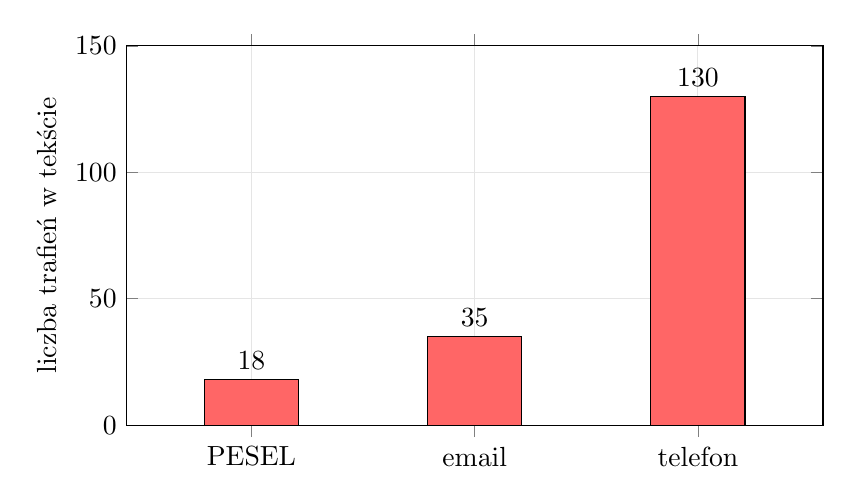
\begin{tikzpicture}
    \begin{axis}[
        ybar,
        width=0.86\linewidth, height=6.4cm,
        ylabel={liczba trafień w tekście},
        symbolic x coords={PESEL, email, telefon},
        xtick=data,
        nodes near coords,
        ymin=0, ymax=150,
        bar width=34pt,
        enlarge x limits=0.28,
        grid=both, grid style={gray!20},
    ]
      \addplot[fill=red!60, draw=black] coordinates {(PESEL,18) (email,35) (telefon,130)};
    \end{axis}
  \end{tikzpicture}
  \caption{\textbf{Bramka gryzie realne dane.} Audyt \texttt{dsbench} na 2211 realnych
  dokumentach SpeakLeash (strided slice shardu \texttt{\_0001}, 6 źródeł). Wykryto
  \textbf{18 PESEL} (poziom \emph{error} $\to$ werdykt FAIL) oraz 35 adresów e-mail i
  130 potencjalnych telefonów (poziom \emph{warn}). Dane realne, nie przykładowe ---
  to dowód, że bramka nie jest atrapą: odrzuca zatrutą kompilację, zanim trafi do treningu.}
  \label{fig:hero}
\end{figure}

\vfill
{\small Slayer \textperiodcentered{} dokument kompilowany w CI do PDF \textperiodcentered{} matematyka w \texttt{\$...\$} \textperiodcentered{} warsztat dialektyczny: \texttt{docs/}}
\end{titlepage}
